\documentclass[border=10pt,tikz]{standalone}
\usepackage{tikz}
\usetikzlibrary{positioning,arrows.meta,shapes}
\begin{document}
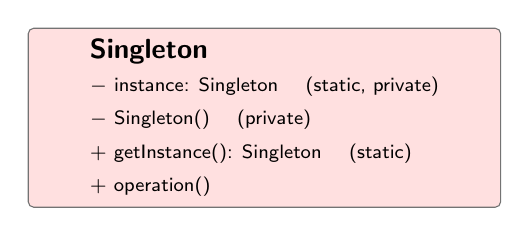
\begin{tikzpicture}[
  font=\sffamily\small,
  cls/.style={rectangle, rounded corners=2pt, draw=black!55, line width=0.4pt,
              minimum height=8mm, minimum width=60mm, inner sep=4pt, fill=red!12, align=left}
]
\node[cls, font=\sffamily\bfseries] (s) at (0,0) {Singleton \\
  \mdseries\scriptsize $-$ instance: Singleton \quad (static, private) \\
  \mdseries\scriptsize $-$ Singleton() \quad (private) \\
  \mdseries\scriptsize $+$ getInstance(): Singleton \quad (static) \\
  \mdseries\scriptsize $+$ operation()
};
\end{tikzpicture}
\end{document}
